\documentclass{beamer}

\usepackage{amssymb,amsmath}
\usepackage{graphicx}
\usepackage{url}
\usepackage{color}
\usepackage{pagenote}[continuous,page]
\usepackage{relsize}		% For \smaller
\usepackage{url}			% For \url
\usepackage{epstopdf}	% Included EPS files automatically converted to PDF to include with pdflatex

%For MindMaps
% \usepackage{tikz}%
% \usetikzlibrary{mindmap,trees,arrows}%

%%% Color Definitions %%%%%%%%%%%%%%%%%%%%%%%%%%%%%%%%%%%%%%%%%%%%%%%%%%%%%%%%%
%\definecolor{bordercol}{RGB}{40,40,40}
%\definecolor{headercol1}{RGB}{186,215,230}
%\definecolor{headercol2}{RGB}{80,80,80}
%\definecolor{headerfontcol}{RGB}{0,0,0}
%\definecolor{boxcolor}{RGB}{186,215,230}

%%% Save space in lists. Use this after the opening of the list %%%%%%%%%%%%%%%%
%\newcommand{\compresslist}{
%	\setlength{\itemsep}{1pt}
%	\setlength{\parskip}{0pt}
%	\setlength{\parsep}{0pt}
%}

%\setbeameroption{show notes on top}

% You should run 'pdflatex' TWICE, because of TOC issues.

% Rename this file.  A common temptation for first-time slide makers
% is to name it something like ``my_talk.tex'' or
% ``john_doe_talk.tex'' or even ``discrete_math_seminar_talk.tex''.
% You really won't like any of these titles the second time you give a
% talk.  Try naming your tex file something more descriptive, like
% ``riemann_hypothesis_short_proof_talk.tex''.  Even better (in case
% you recycle 99% of a talk, but still want to change a little, and
% retain copies of each), how about
% ``riemann_hypothesis_short_proof_MIT-Colloquium.2000-01-01.tex''?

\mode<presentation>
{
  \usetheme{CambridgeUS}		% bem bacana - menu superior
  \usecolortheme{default}		% branco, azul clarinho
  \useoutertheme{default}
  \useinnertheme{circles}
  \setbeamercovered{invisible}
}

\beamertemplatenavigationsymbolsempty

%% Better looking blocks
\setbeamercolor{block title alerted}{use=structure,fg=black,bg=red!80!black}
\setbeamercolor{block body alerted}{use=structure,fg=black,bg=white!90!black}

\setbeamercolor{block title}{use=structure,fg=black,bg=blue!60!white}
\setbeamercolor{block body}{use=structure,fg=black,bg=white!90!black}

\usepackage[english]{babel}
\usepackage[latin1]{inputenc}
\usepackage{subfigure}

\usepackage{times}
\usepackage[T1]{fontenc}

%% makes the ppagenote command for figure references at the end.
\makepagenote
\renewcommand{\notenumintext}[1]{}
\newcommand{\ppagenote}[1]{\pagenote[Page \insertframenumber]{#1}}


\usepackage{tikz}
\usetikzlibrary{arrows,shapes}

\title[GB13604]{GB13604 - Maths for Computer Science}
\subtitle[]{Lecture 9 -- Probability, Part II}
\author[Claus Aranha]{Claus Aranha\\{\footnotesize caranha@cs.tsukuba.ac.jp}}
\institute[COINS]{College of Information Science}
\date[2018-12-12]{2018-12-12\\{\tiny Last updated \today}}

\tikzstyle{vertex}=[circle,fill=black!25,minimum size=10pt,inner sep=0pt]
\tikzstyle{blue vertex}=[circle,fill=blue!100,minimum size=10pt,inner sep=0pt]
\tikzstyle{red vertex}=[circle,fill=red!100,minimum size=10pt,inner sep=0pt]
\tikzstyle{yellow vertex}=[circle,fill=yellow!100,minimum size=10pt,inner sep=0pt]
\tikzstyle{edge} = [draw,thick,-]
\tikzstyle{pedge} = [draw,thick,.]
\tikzstyle{red edge} = [draw, thick,-,red!50]
\tikzstyle{black edge} = [draw, line width=2pt,-,black!20]
\tikzstyle{weight} = [font=\smaller]

\begin{document}

\begin{frame}
  \maketitle

  \begin{center}
    {\smaller This course is based on Mathematics for Computer Science, Spring
    2015, by Albert Meyer and Adam Chlipala, Massachusetts Institute
    of Technology OpenCourseWare.}
    
    
\includegraphics[width=0.2\textwidth]{../img/by-nc-sa}
  \end{center}
\end{frame}

\begin{frame}
  \frametitle{Introduction}
  \begin{itemize}
  \item Independence and Causality
  \item Random Variables
  \item Expectation
  \end{itemize}
\end{frame}

\section{Independence and Causality}

\begin{frame}

  \begin{center}
    {\huge
      Independence and Causality
    }
  \end{center}
\end{frame}

\subsection{Basics}

\begin{frame}
  \frametitle{Independent Events}

  \begin{itemize}
  \item If it is raining, the probability that people will take the
    bus from tsukuba station is higher than if it is sunny.

    \begin{equation*}
      \text{Pr(Take the bus | raining)} \neq \text{Pr(Take the bus | sunny)}
    \end{equation*}
    \bigskip

  \item If your father and mother have type A blood, the probability
    that you have type A blood is higher.
    \begin{equation*}
      \text{Pr}(A_{me} | A_{P} \& A_{M}) \geq \text{Pr}(A_{me})
    \end{equation*}
    \bigskip
    
  \item If you flip two separate coins, the probability of the second
    coin being heads is not influenced by the result of the first
    coin.
    \begin{equation*}
      \text{Pr}(H_2 | H_1) = \text{Pr}(H_2 | \bar{H_1}) = \text{Pr}(H_2)
    \end{equation*}
  \end{itemize} 
\end{frame}

\begin{frame}
  \frametitle{Independent Events}

  Two events, \structure{A} and \structure{B} are \structure{independent} if the
  probability of A \structure{does not depend} on the occurrence of B.

  \bigskip

  {\bf Mathematical Definitions:}
  \begin{itemize}
  \item {\bf Definition 1:} Events \structure{A} and \structure{B} are
    \structure{independent} {\bf iff}:
    \begin{equation}
      \text{Pr}(A) = \text{Pr}(A|B)
    \end{equation}
  \item {\bf Definition 2:} Events \structure{A} and \structure{B} are
    \structure{independent} {\bf iff}:
    \begin{equation}
      \text{Pr}(A)\cdot\text{Pr}(B) = \text{Pr}(A\cap B)
    \end{equation}
  \end{itemize}
\end{frame}

\begin{frame}
  \frametitle{Proof of Equivalence of Definitions 1 and 2}

  Definition 1:
  \begin{equation*}
    \text{Pr}(A) = \text{Pr}(A|B) \text{ {\bf iff}}
  \end{equation*}

  \bigskip

  Conditional Prob Definition:
  \begin{equation*}
    \text{Pr}(A) = \frac{\text{Pr}(A \cap B)}{\text{Pr}(B)} \text{ {\bf iff}}
  \end{equation*}

  \bigskip

  Algebra:
  \begin{equation*}
    \text{Pr}(A)\cdot\text{Pr}(B) = \text{Pr}(A \cap B).
  \end{equation*}
\end{frame}

\begin{frame}
  \frametitle{Independence: Characteristics}

  {\bf Simmetry:}
  \begin{equation*}
    \text{Pr}(A)\cdot\text{Pr}(B) = \text{Pr}(A \cap B).
  \end{equation*}
  If $A$ is independent from $B$, \alert{then} $B$ is independent from $A$.

  \vfill

  {\bf Zero probability event:}\\
  If Pr$(B) = 0$ then:
  \begin{itemize}
  \item {\bf Definition 1:} Does not work
  \item {\bf Definition 2:} $\text{Pr}(A)\cdot0 = \text{Pr}(A \cap
    \emptyset) = 0$.
  \end{itemize}
  So, $B$ is \alert{independent from all events}!
\end{frame}

\begin{frame}
  \frametitle{Independence: Complement}

  \structure{A independent of B} means probability of A does not
  change \alert{if B happens or not}. {\bf Therefore} A should also be
  independent of {\bf Not B}.

  \vfill
  {\bf Lemma:} A independent of B {\bf iff} A independent of NOT B.

  \vfill
  
  {\bf Proof:} Proof can be derived using algebra from:
  \begin{equation*}
    \text{Pr}(A-B) = \text{Pr}(A)-\text{Pr}(A\cap B)
  \end{equation*}
\end{frame}

\subsection{Mutual Independence}

\begin{frame}
  \frametitle{Mutual Independence: Idea}

  {\bf Experiment:} Two coins are thrown
  \begin{itemize}
  \item {\bf Event 1}: Coin 1 is heads: Pr$(H_1) = (0,0),(0,1),(1,0),(1,1) = 0.5$
  \item {\bf Event 2}: Coin 2 is heads: Pr$(H_2) = (0,0),(0,1),(1,0),(1,1) = 0.5$
  \item {\bf Event 3}: \# of heads is odd: Pr$(O) = (0,0),(0,1),(1,0),(1,1) = 0.5$
  \end{itemize}

  \vfill

  \begin{onlyenv}<2>
  Events $H_1,H_2$, $H_1,O$, $H_2,O$ are, \alert{2-by-2}, independent:
  \begin{itemize}
  \item Pr$(O|H_1) = (1,0), (1,1) = 0.5$
  \item Pr$(O|H_2) = (0,1), (1,1) = 0.5$
  \item Pr$(H_1|H_2) = (0,1), (1,1) = 0.5$
  \end{itemize}

  \bigskip

  These 3 events are \structure{2-way independent}.
  \end{onlyenv}
\end{frame}

\begin{frame}
  \frametitle{Mutually Independent Events -- Definition}

  Events $A_1, A_2, A_3, \ldots, A_n$ are \structure{Mutually
    Independent} when:

  \vfill
  
  The probability that $A_i$ occurs is not changed by the occurence of
  the other events.
\end{frame}

\begin{frame}
  \frametitle{Mutually Independent Events -- Example}

  {\bf Experiment:} You throw the coin $n$ times\\
  {\bf Event:} $H_i$ the $i$-th throw is \structure{heads}

  \vfill

  What happens in the 5th flip is independent from the 1st flip, or
  the 7th flip, etc.

  \bigskip
  
  \begin{equation*}
    \text{Pr}(H_5) = \text{Pr}(H_5|H_1 \cap H_3 \cap H_7 \cap \ldots)
  \end{equation*}
\end{frame}

\begin{frame}
  \frametitle{Mutiually Independent Events -- Math Def}

  Events $A_1, A_2, \ldots A_n$ are \structure{mutually independent} when:

  \vfill
  
  {\bf Definition 1:}
  \begin{equation}
    \text{Pr}(A_i) = \text{Pr}(A_i|A_1 \cap A_2 \cap \ldots \cap A_j \cap  \ldots \cap A_n); j \neq i
  \end{equation}

  \bigskip
  
  {\bf Definition 2:}
  \begin{equation}
    \text{Pr}(A_1 \cap A_2 \cap A_3 \cap \ldots \cap A_n) = \text{Pr}(A_1)\cdot\text{Pr}(A_2)\cdot\text{Pr}(A_3)\cdot\ldots\cdot\text{Pr}(A_n) 
  \end{equation}
\end{frame}

\begin{frame}
  \frametitle{K-wise independence}

  {\bf Experiment:} Two coins are thrown
  \begin{itemize}
  \item {\bf Event 1}: Coin 1 is heads: Pr$(H_1) = (0,0),(0,1),(1,0),(1,1) = 0.5$
  \item {\bf Event 2}: Coin 2 is heads: Pr$(H_2) = (0,0),(0,1),(1,0),(1,1) = 0.5$
  \item {\bf Event 3}: \# of heads is odd: Pr$(O) = (0,0),(0,1),(1,0),(1,1) = 0.5$
  \end{itemize}

  \vfill
  
  \begin{itemize}
  \item Each pair $(H_1, H_2),(H_1,O),(H_2,O)$ is mutually independent.
  \item However, $(H_1, H_2, O)$ are not mutually independent:
    Pr$(O|H_1\cap H_2) = 0$
  \end{itemize}
\end{frame}

\begin{frame}
  \frametitle{K-wise independence}
  {\larger
  {\bf Experiment:} $n$ coins are thrown
  \begin{itemize}
  \item {\bf Event i}: Coin i is heads: Pr$(H_i) = 0.5$
  \item {\bf Event $i+1$}: \# of heads is odd: Pr$(O) = 0.5$
  \end{itemize}

  \vfill
  
  \structure{Any subset of $i$ events} is mutually independent.\\
  However, \alert{the set of all $i+1$} events is {\bf not}.
  }  
\end{frame}

\begin{frame}
  \frametitle{K-wise independence}

  {\larger
    A set of $m$ events is $k$-wise independent if:

    \bigskip
    
    $A_1, A_2, \ldots, A_m$

    \bigskip

    Any subset of $k$ events is mutually independent.
  }             
\end{frame}

\section{Random Variables}

\begin{frame}
  \begin{centering}
    {\huge
      Random Variables
    }
  \end{centering}
\end{frame}

\subsection{Intuitive Example}
\begin{frame}
  \frametitle{Playing tRPGs}

  \begin{columns}
    \column{0.7\textwidth}
    In the game \structure{3:16}, you \alert{win a space battle} if you
    roll a d10 dice, and the result is below the value \structure{FA},
    which you decide before the game.
    
    \bigskip
    
    \begin{itemize}
    \item If you lose one battle \alert{you lose your armor}
    \item If you lose another battle \alert{you are wounded}
    \item If you lose a third battle \alert{you die}
    \end{itemize}
    \column{0.3\textwidth}
    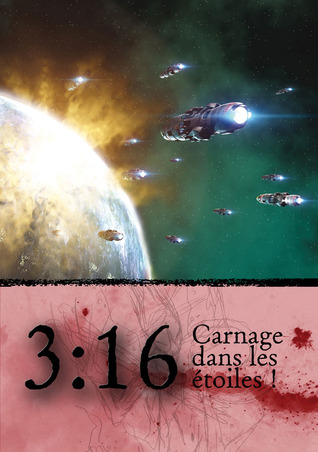
\includegraphics[width=1\textwidth]{../img/316}
  \end{columns}  
\end{frame}

\begin{frame}
  \frametitle{Events and Numbers}

  Until now, we approached probability from a \structure{Set} and
  \structure{Events} point of view:
  \begin{itemize}
  \item {\bf Event 1:} Result of the dice: $\{1,2,3,4,5,6,7,8,9,10\}$
  \item {\bf Event 2:} Value of {\bf FA}: $\{1,2,3,4,5,6,7,8,9,10\}$
  \item {\bf Event 3:} You win a combat with FA = 6:\\
    $\{1,6\}, \{2,6\}, \{3,6\}, \ldots$
  \item {\bf Event 4:} 3 victories in 5 battles with FA = 6:\\ $\{E_3,
    E_3, E_3, \bar{E_3}, \bar{E_3}\}, \{E_3, E_3, \bar{E_3}, E_3,
    \bar{E_3}\}, \ldots$
  \end{itemize}
\end{frame}

\begin{frame}
  \frametitle{Events and Numbers}

  However, many times we want to see probability in terms of
  \structure{Numbers}:
  \begin{itemize}
  \item What is the probability that I can \alert{survive 7 battles}
    if my FA is 6?
  \item What is the \alert{minimum FA} I need to have more than .8
    chance to survive 5 battles?
  \item \alert{How many battles in a row} I expect to win if my FA is 6?
  \end{itemize}

  \vfill
  
  Intuitively, a \structure{Random Variable} is a number that comes from
  a \structure{Random Process}
  \begin{itemize}
  \item \# of hours to the next \structure{System Crash}
  \item \# \structure{faulty pixels} in the monitor
  \item \# heads in a \structure{coin flip}
  \end{itemize}
\end{frame}

\subsection{Random Variable: Definition}
\begin{frame}
  \frametitle{Random Variable: Formal Definition}

  A random variable is a \structure{total function} from a
  \structure{sample space} to a \structure{numeric domain}.

  \bigskip
  \begin{equation}
    R: S \to \mathbb{R} \text{ or } R: S \to \mathbb{N}, \text{ etc...}
  \end{equation}

  \vfill

  So a random \emph{variable} is really a \alert{function}...\\
  \hfill (... maybe that is a bad name)
\end{frame}

\begin{frame}
  \frametitle{Random Variable: Formal Example}

  {\bf Experiment}: We throw three \emph{fair} coins independently.
  \begin{itemize}
  \item Variable $C$ ::= Number of heads ({\bf C}ount)
  \item Variable $M$ ::= 1 if all coins {\bf M}atch, 0 if they don't {\bf M}atch
  \end{itemize}

  \vfill

  \begin{itemize}
  \item $M = 1$ when $\{H,H,H\}$ or $\{T,T,T\}$, \\
    Pr$(M=1) = 2/8$
    \bigskip
    
  \item $C = 1$ when $\{H,T,T\},\{T,H,T\},\{T,T,H\}$, \\
    Pr$(C=1) = 3/8$
    \bigskip

  \item Pr$(C\cdot M > 0) = \text{Pr}(C>0 \cap M>0) = 1/8$
  \end{itemize}
\end{frame}


\begin{frame}
  \frametitle{``Indicator'' random variables}

  An {\bf indicator random variable} \structure{takes a value of 0 or 1} for
  a subset of the sample space.
  \begin{itemize}
  \item Variable $M$ ::= 1 if all coins {\bf M}atch, 0 if they don't {\bf M}atch
    \bigskip

  \item Variable $O$ ::= 1 if number of heads is {\bf O}dd.    
  \end{itemize}

  \vfill
  
  Other \structure{integer} random variables \structure{partition} the
  sample space:
  \begin{itemize}
  \item $C = 0 \to \{T,T,T\}$
  \item $C = 1 \to \{H,T,T\}, \{T,H,T\}, \{T,T,H\}$
  \item $C = 2 \to \{H,T,H\}, \{H,H,T\}, \{T,H,H\}$
  \item $C = 3 \to \{H,H,H\}$
  \end{itemize}
\end{frame}

\subsection{Independence}
\begin{frame}
  \frametitle{Independence and Random Variables}

  So, a \structure{Random Variable} is a \alert{function} that assigns
  a value to a set of outcomes.

  \bigskip

  Two or more \structure{Random Variables} $R_1, R_2, \ldots, R_n$ are
  mutually independent {\bf iff} $(R_1 = a_1), (R_2 = a_2), \ldots,
  (R_n = a_n)$ are all \structure{mutually indepedent events}.

  \bigskip

  {\bf Alternatively:}\\
  \begin{equation*}
    \text{Pr}(R_1 = a_1 \cap R_2 = a_2 \cap R_3 = a_3 \cap \ldots) =
    \text{Pr}(R_1 = a_1)\cdot\text{Pr}(R_2 = a_2)\ldots
  \end{equation*}
  \hfill For all values of $a_1$
\end{frame}

\begin{frame}
  \frametitle{Independence and Random Variables}

  Are R.V.s $C$ and $M$ independent?
  \bigskip
  
  \begin{itemize}
  \item Variable $M$ ::= 1 if all coins {\bf M}atch, 0 if they don't {\bf M}atch
  \item Variable $C$ ::= number of heads ({\bf C}ount).    
  \end{itemize}

  \bigskip

  {\bf Answer:} \alert{NO!}
  \begin{itemize}
  \item Pr$(M=1)\cdot$Pr$(C=1) > 0$
  \item Pr$(M=1 \cap C=1) = 0$
  \end{itemize}  
\end{frame}

\begin{frame}
  \frametitle{Independence and Random Variables}

  Are R.V.s $O$ and $M$ independent?
  \bigskip
  
  \begin{itemize}
  \item Variable $M$ ::= 1 if all coins {\bf M}atch, 0 if they don't {\bf M}atch
  \item Variable $O$ ::= 1 if \# heads is {\bf O}dd, 0 if it is even.    
  \end{itemize}

  \bigskip

  {\bf Answer:} \structure{YES!}
  \begin{itemize}
  \item Pr$(M=1)\cdot$Pr$(O=1) = \frac{2}{8}\cdot\frac{1}{2} = \frac{1}{8}$
  \item Pr$(M=1 \cap C=1) = \frac{1}{8}$
    \bigskip
    
  \item Don't forget to test for the other combinations: $(M = 0, C = 1), (M = 1, C = 0), \ldots$

    \bigskip

  \item To prove \alert{NOT} independence, you just need one counterexample.
  \end{itemize}  
\end{frame}

\subsection{PDF and CDF}

\begin{frame}
  \frametitle{Uniform Random Variables}

  A \structure{Uniform} Random Variable is one where the \structure{all values are equally likely}.

  \vfill

  \begin{itemize}
  \item $D_n$ ::= result of a \structure{fair} dice with $n$ sides.
    \begin{equation*}
      \text{Pr}(D_6 = 1) = \text{Pr}(D_6 = 2) = \ldots = \text{Pr}(D_6 = 6) =
      \frac{1}{6}
    \end{equation*}
    \bigskip

  \item $S_4$ ::= lottery number with 4 digits.
    \begin{equation*}
      \text{Pr}(S_4 = 0000) = \text{Pr}(S_4 = 1234) = \ldots =
      \text{Pr}(S_4 = 9998) = 0.0001
    \end{equation*}
  \end{itemize}
  
\end{frame}

\begin{frame}
  \frametitle{Binomial Random Variable}

  {\bf Experiment:} We throw a biased coin $n$ times, each time with
  $p$ chance to turn heads.
  \bigskip

  {\bf Event:} $B_{n,p}$::= \# of heads in $n$ mutually independent
  flips.

  \vfill

  For $n = 5, p = 2/3$, Pr$(HHTTH)$:
  \begin{itemize}
  \item<2-> = Pr$(H)\cdot$Pr$(H)\cdot$Pr$(T)\cdot$Pr$(T)\cdot$Pr$(H)$
  \item<3-> $=
    \frac{2}{3}\cdot\frac{2}{3}\cdot\frac{1}{3}\cdot\frac{1}{3}\cdot\frac{2}{3}$
  \item<4-> $= \frac{2}{3}^3\cdot\frac{1}{3}^2$
  \end{itemize}
\end{frame}

\begin{frame}
  \frametitle{Binomial Random Variable}

  {\bf Experiment:} We throw a biased coin $n$ times, each time with
  $p$ chance to turn heads.
  \bigskip

  {\bf Event:} $B_{n,p}$::= \# of heads in $n$ mutually independent
  flips.

  \vfill

  For $n = 5, p = 2/3$:
  \begin{itemize}
  \item Pr(\structure{ONE seq with i $H$ and (n-i) $T$}):\\
    $p^i(1-p)^{n-i}$
    \bigskip
    
  \item Pr(\structure{ANY seq with i $H$ and (n-i) $T$}):\\
    $\binom{n}{i}p^i(1-p)^{n-i}$
  \end{itemize}
\end{frame}

\begin{frame}
  \frametitle{Probability Density Function}
  
  The \structure{Probability Density Function (PDF)} of a random variable $R$
  defines the probability that $R$ will have a given value $i$
  \bigskip

  \begin{equation*}
    \text{PDF}_R(i) ::= \text{Pr}(R = i)
  \end{equation*}
  \bigskip
  
  {\bf Example 1:} for the binomial random variable:
  \begin{equation*}
    \text{PDF}_{B_{n,p}}(i) = \binom{n}{i}p^i(1-p)^{n-i}
  \end{equation*}
  \bigskip
  
  {\bf Example 2:} for the uniform random variable:
  \begin{equation*}
    \text{PDF}_{U}(v) = \text{constant}
  \end{equation*}
  \hfill (for $v$ in range of $U$)
\end{frame}

\begin{frame}
  \frametitle{Cumulative Distribution}

  The \structure{Cumulative Distribution Function} is the function that
  measures the probability that random variable $R$ will have a value
  \structure{smaller or equal} than $i$
  \bigskip

  \begin{equation*}
    \text{CDF}_R(i) ::= \text{Pr}(R \leq i)
  \end{equation*}
  \vfill

  {\bf Important points}
  \begin{itemize}
  \item PDF and CDF capture similar information.
  \item PDF and CDF \structure{do not involve} the actual sample space.
  \item Many different {\bf experiment} have \structure{very similar PDFs}
  \end{itemize}
\end{frame}

\begin{frame}
  \frametitle{PDF and CDF example: 2d6}
  \begin{center}
    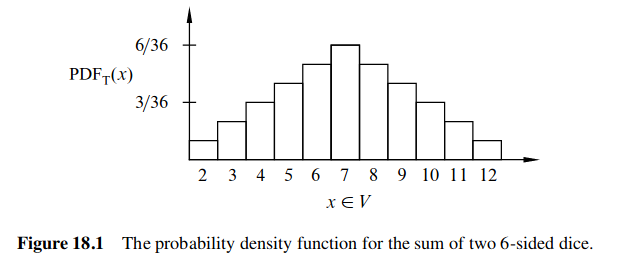
\includegraphics[height=0.4\textheight]{../img/pdf_2d6}
    \bigskip

    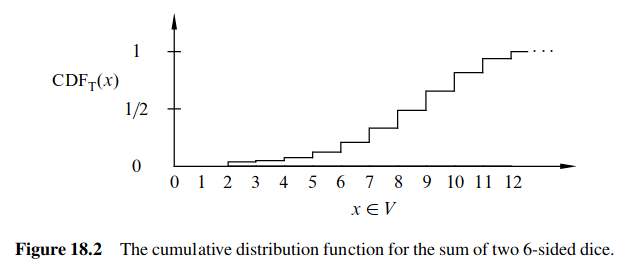
\includegraphics[height=0.4\textheight]{../img/cdf_2d6}
  \end{center}
\end{frame}

\section{Expectation}
\begin{frame}
  \begin{center}
    {\huge
      Expectation
    }
  \end{center}
\end{frame}

\begin{frame}
  \frametitle{Game: Carnival Dice}

  Consider the following game: \structure{Choose a number of 1 to 6}
  and roll \alert{3 dice}. Each dice that \structure{rolls the same number}
  you win \$1. If \alert{no dice} roll that number, you lose \$1.

  \bigskip

  {\bf Example:} You choose \alert{number 5}:
  \begin{itemize}
  \item<2-> 2, 3, 4: \alert{Lose \$1}
  \item<3-> {\bf 5}, 4, 6: \structure{Win \$1}
  \item<4-> {\bf 5}, {\bf 5}, 1: \structure{Win \$2}
  \item<5-> {\bf 5}, {\bf 5}, {\bf 5}: \structure{Win \$3}
    \bigskip
    
  \item<6> Is this a fair game?
  \end{itemize}  
\end{frame}

\begin{frame}
  \frametitle{Game: Carnival Dice Analysis}

  {\larger
  \begin{itemize}
  \item Pr(zero 5s) = $\frac{5}{6}^3 = \frac{125}{216}$ = \alert{Lose \$1}
    \bigskip
    
  \item Pr(one 5) = $\binom{3}{1}\frac{5}{6}^2\frac{1}{6} =
    \frac{75}{216}$ = \structure{Win \$1}
    \bigskip
    
  \item Pr(two 5) = $\binom{3}{2}\frac{5}{6}\frac{1}{6}^2 =
    \frac{15}{216}$ = \structure{Win \$2}
    \bigskip
    
  \item Pr(three 5) = $\frac{1}{6}^3 = \frac{1}{216}$ = \structure{Win
    \$3}
  \end{itemize}
  }
\end{frame}

\begin{frame}
  \frametitle{Carnival Game: Law of Averages}

  Every \alert{216 Games}, you expect \alert{125 games} with 0
  matches, \alert{75 games} with 1 match, \alert{15 games} with 2
  matches, and only \alert{one game} with 3 matches!

  \bigskip

  \begin{equation*}
    \frac{216\times(-1)+75\times(1)+15\times(2)+1\times(3)}{216} = \frac{-17}{216} = -0.08
  \end{equation*}

  \bigskip

  So on average, you expect to \alert{lose \$0.08} per game. Not a fair game!
\end{frame}

\begin{frame}
  \frametitle{Carnival Game: Impossible expectations}

  Note that, for the carnival game, you \alert{expect to lose 0.08 per
    game} but {\bf the result -0.08 does not exist!}

  \vfill

  {\bf Another example:} Rolling one 6-sided die:
  \bigskip

  Pr(1) = 1/6, Pr(2) = 1/6, Pr(3) = 1/6, $\ldots$
  \bigskip

  \begin{equation*}
    \text{Expected value } = \frac{1\cdot1 + 1\cdot2 + 1\cdot3 + 1\cdot4 + 1\cdot5 + 1\cdot6}{6} = \frac{21}{6} = 3.5 
  \end{equation*}
  You expect an \structure{average result} of 3.5, but the 3.5 result
  does not exist!
\end{frame}

\begin{frame}
  \frametitle{Expectation: Definitions}

  The \structure{Expected Value} of a variable $R$ is the
  \structure{Average Value} of $R$, weighted by the probabilities.

  \bigskip

  \begin{equation}
    E[R] ::= \sum_{v \in \text{range}(R)}v\cdot\text{Pr}[R = v]
  \end{equation}

  \bigskip
  So, $E[\$ \text{ at carnival game}] = -0.08$

  \vfill

  {\bf Note 1:} We can use sums in this definition because the
  \structure{probability space is countable}.\\
  {\bf Note 2:} For \structure{continuous probability spaces} we need
  to use integrals.
\end{frame}

\begin{frame}
  \frametitle{Total Expectation}

  \structure{Law of Total Expectation} is useful for reasoning by cases:
  \bigskip

  \begin{itemize}
  \item {\bf Conditional Expectation:} $E[R|A] = \sum v\cdot\text{Pr}[R = v|A]$
    \bigskip

  \item {\bf Total Expectation:} $E[R] = E[R|A]\cdot\text{Pr}[A] +
    E[R|\bar{A}]\cdot\text{Pr}[\bar{A}]$
  \end{itemize}

  \bigskip

  In other words: The total expectation is \structure{The expectation
    when $A$ happens} plus \structure{The expectation when $A$ does
    not happen}.
\end{frame}

\begin{frame}
  \frametitle{General Total Expectation}

  More generally:
  \bigskip

  \begin{equation}
    E[R] = E[R|A_1]\cdot\text{Pr}[A_1] + E[R|A_2]\cdot\text{Pr}[A_2] +
    \ldots + E[R|A_n]\cdot\text{Pr}[A_n]
  \end{equation}
  \bigskip

  when $\text{Pr}[A_1] + \text{Pr}[A_2] + \ldots + \text{Pr}[A_n] = 1$
\end{frame}

\begin{frame}
  \frametitle{Total Expectation: How many heads?}

  What is \structure{expected number of Heads} when we flip a coin $n$
  times with \alert{bias p}?

  \bigskip
  A coin with \alert{bias p}:
  \begin{itemize}
  \item Will turn {\bf Heads} with probability $p$
  \item Will turn {\bf Tails} with probability $q = 1-p$ 
  \end{itemize}

  \vfill
  
  $E[n]$ expectation of heads after $n$ flips - \structure{study by cases}:
  \begin{itemize}
  \item {\bf Case 1:} First coin is Heads: $E[n|H_1] = 1 + E[n-1]$
  \item {\bf Case 2:} First coin is Tails: $E[n|T_1] = E[n-1]$
  \end{itemize}
\end{frame}

\begin{frame}
  \frametitle{Total Expectation: How many heads?}

  $E[n]$ expectation of heads after $n$ flips - \structure{study by cases}:
  \begin{itemize}
  \item {\bf Case 1:} First coin is Heads: $E[n|H_1] = 1 + E[n-1]$
  \item {\bf Case 2:} First coin is Tails: $E[n|T_1] = E[n-1]$
  \end{itemize}

  \bigskip

  By \structure{total expectation}:
  \begin{itemize}
  \item<2-> $E[n] = E[n|H_1]\cdot p + E[n|T_1]\cdot q$
  \item<3-> $E[n] = (1+E[n-1])\cdot p + (E[n-1])\cdot q$
  \item<4-> $E[n] = p + E[n-1](p+q) = p + E[n-1]$
  \item<5-> $E[n] = p + E[n-1] = p + p + E[n-2] = 3p + E[n-3] = np + E[0] = np$
  \end{itemize}
\end{frame}

\subsection{Mean Time To Failure}
\begin{frame}
  \frametitle{Mean Time To Failure}

  Suppose that a computer has a \structure{chance to fail} of $p$ every hour.

  \bigskip
  
  \begin{center}
    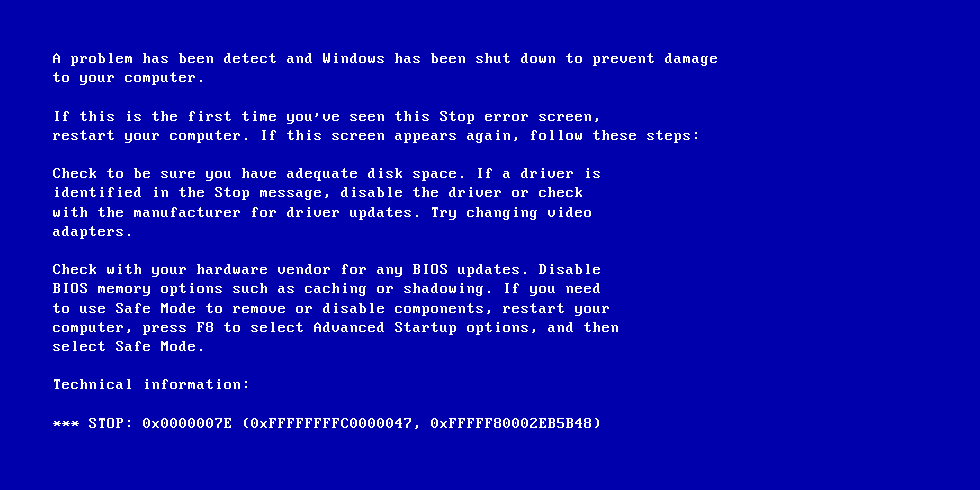
\includegraphics[width=0.7\textwidth]{../img/bsod}
  \end{center}

  \bigskip

  \alert{How many hours} does it take for the computer to fail on average?
\end{frame}

\begin{frame}
  \frametitle{Mean Time To Failure}

  \begin{itemize}
  \item Chance to fail \alert{in the first hour} = $p$
  \item Chance to fail \alert{in the second hour} = $qp$
  \item Chance to fail \alert{in the third hour}  = $q^2p$
  \item $\ldots$
  \item Chance to fail \alert{in the n-th hour} = $q^{n-1}p$
  \end{itemize}

  \vfill

  \begin{center}
    {\bf Geometric Distribution / Geometric Sum}
  \end{center}
  
\end{frame}

\begin{frame}
  \frametitle{Mean Time To Failure}

  \alert{How many hours} does it take for the computer to fail on
  average?

  \bigskip
  
  \begin{itemize}
  \item $E[F] = \sum_{n>0}n\cdot\text{Pr}[F = n]$
    \bigskip
    
  \item $E[F] = \sum_{n>0}nq^{n-1}p = p\sum_{n>0}nq^{n-1}$
    \bigskip
    
  \item $E[F] = p\cdot\frac{1}{(1-q)^2}$
    \bigskip
    
  \item $E[F] = p\cdot\frac{1}{p^2} = \frac{1}{p}$
  \end{itemize}

  So, in average, the server will fail after $\frac{1}{p}$ hours.
\end{frame}

% TODO: Linearity of Expectation

\section{Conclusion}

\begin{frame}
  \frametitle{Class Summary}
  \begin{itemize}
  \item \structure{Random Variable} is a total function that describes
    a numeric value for a set of probability events.
    \bigskip
    
  \item \structure{Probability Density Function} describes the
    probability of a Random Variable to have a certain value $a$
    \bigskip

  \item \structure{Expectation} is the weighted average of a PDF over
    its domain.    
  \end{itemize}
\end{frame}

\begin{frame}
  \frametitle{Next Class}
  \begin{itemize}
  \item No Exercise Sheet for Next class!
    \bigskip
    
  \item Sample Exam;
    \bigskip

  \item Lecture Evaluation;
  \end{itemize}

  \vfill

  \begin{center}
    Please come!
  \end{center}
\end{frame}

\end{document}
